\section{Feature Selection}
In this section, the focus is on identifying the optimal number of features for different types of audio features (MFCC, Chroma, CQT, etc.).
Each type of feature can consist of a varying number of individual features, and it is crucial to determine the optimal number to maximize
the model's performance. Proper feature selection is vital because it directly impacts the efficiency, accuracy,
and generalizability of the machine learning model. Including too many features can lead to overfitting, increased computational costs,
and degraded performance due to the curse of dimensionality. On the other hand, using too few features can result in underfitting,
where the model fails to capture the necessary patterns in the data. Therefore, the goal of this study is to identify the optimal number of features
for each type to ensure the model is both robust and efficient.

\subsection{Determining the Optimal Number of Features}

To maximize the model's performance, it is crucial to determine the optimal number of features for each type.
This was achieved using a `One Model per Feature' approach, which involved the following steps:

\begin{algorithm}
    \caption{Feature Optimization Process}
    \begin{algorithmic}[1]
        \State \textbf{Step 1:} Extract feature sets with varying sizes: 12, 20, 30, 40, 60, 70, 90, and 120 features.
        \State \textbf{Step 2:} Train a separate model for each feature type and feature set size.
        \State \textbf{Step 3:} For each feature set, train three different models using three classifiers: SVM, Random Forest,
        and Logistic Regression.
        \State \textbf{Step 4:} Evaluate the performance of each model.
    \end{algorithmic}
\end{algorithm}
\noindent
Figure \ref{fig:n_feature_per_type} shows the results obtained for each type of feature with the Random Forest model,
which significantly outperformed the other classifiers.


\begin{figure*}[htbp]
    \centering
    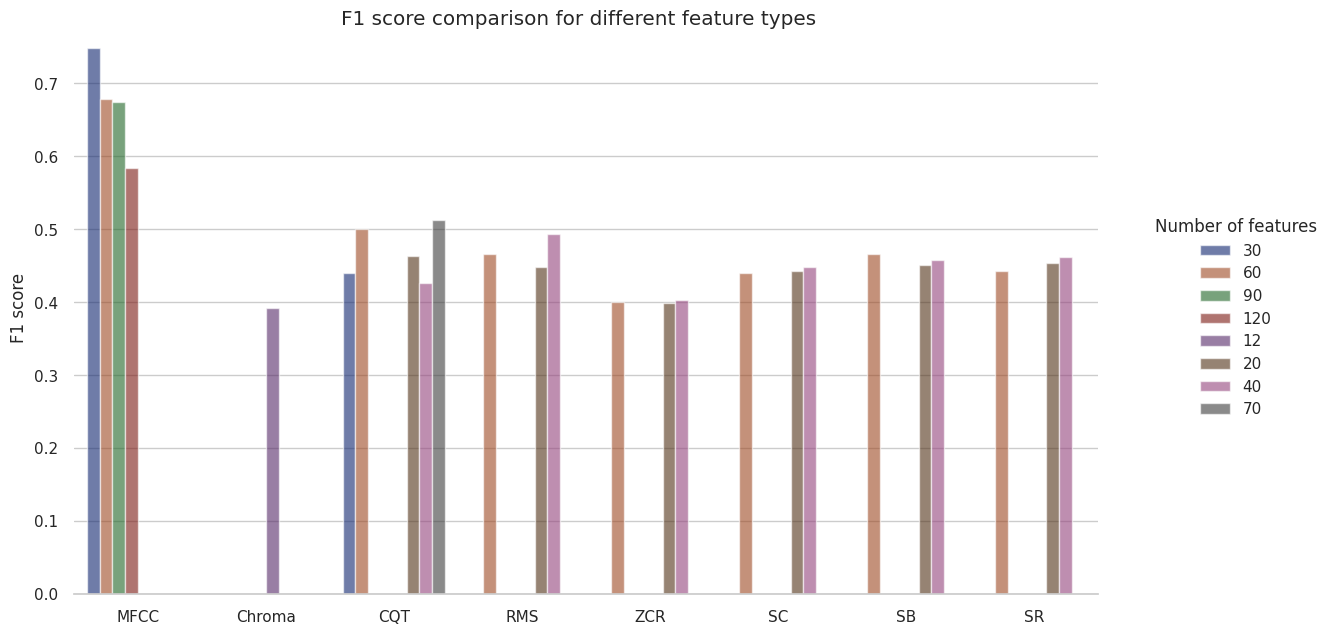
\includegraphics[width=.8\textwidth]{../images/n_feature_per_type.png}
    \caption{F1 score per number of features}
    \label{fig:n_feature_per_type}
\end{figure*}

\subsection{Results and Analysis}

\textbf{MFCC:} The MFCC features consistently achieved the highest F1 scores, peaking around 0.7.
This indicates their effectiveness for the classification task. Interestingly, the number of MFCC features (ranging from 30 to 120)
did not drastically affect performance, suggesting that even a smaller set of MFCC features can be highly informative.\\
\textbf{CQT:} The CQT features showed moderate performance, with F1 scores around 0.4 to 0.5. The optimal number of features was around 70,
beyond which there was no significant improvement.\\
\textbf{RMS:} RMS features exhibited F1 scores ranging from 0.4 to 0.5, with optimal performance achieved with around 70 features.\\
\textbf{ZCR, Spectral Centroid (SC), Spectral Bandwidth (SB), and Spectral Roll-off (SR):}
The F1 scores for these features generally stabilized around 0.4 to 0.5.
Increasing the number of features beyond 40 did not result in significant performance gains and could even degrade the model's performance.
This suggests that adding too many features, especially those without strong predictive power, can confuse the model and degrade its performance.

\subsection{Optimal Number of Features}

Based on the results, the optimal number of features for each type is as follows:
\rowcolors{2}{blue!8}{blue!18}
\begin{table}[h]
    \centering
    \small
    \begin{tabular}{|c|c|}
        \hline
        \textbf{Feature Type} & \textbf{Optimal Number of Features} \\
        \hline
        MFCC                  & 30                                  \\
        Chroma                & 12                                  \\
        CQT                   & 70                                  \\
        RMS                   & 40                                  \\
        ZCR                   & 40                                  \\
        Spectral Centroid     & 40                                  \\
        Spectral Bandwidth    & 60                                  \\
        Spectral Roll-off     & 40                                  \\
        \hline
    \end{tabular}
    \caption{Optimal number of features for each type}
    \label{tab:optimal_features}
\end{table}

